\chapter{Supplementary figures}\label{appx:supplementaryFigures}
\markboth{\spacedlowsmallcaps{A Supplementary figures}}{\spacedlowsmallcaps{A Supplementary figures}}

\section{Momentum data measurements (\SIrange{30}{200}{\femto\s})}

\subsection{Momentum distributions (\SIrange{30}{200}{\femto\s})}

\begin{figure}[H]
  \centering
  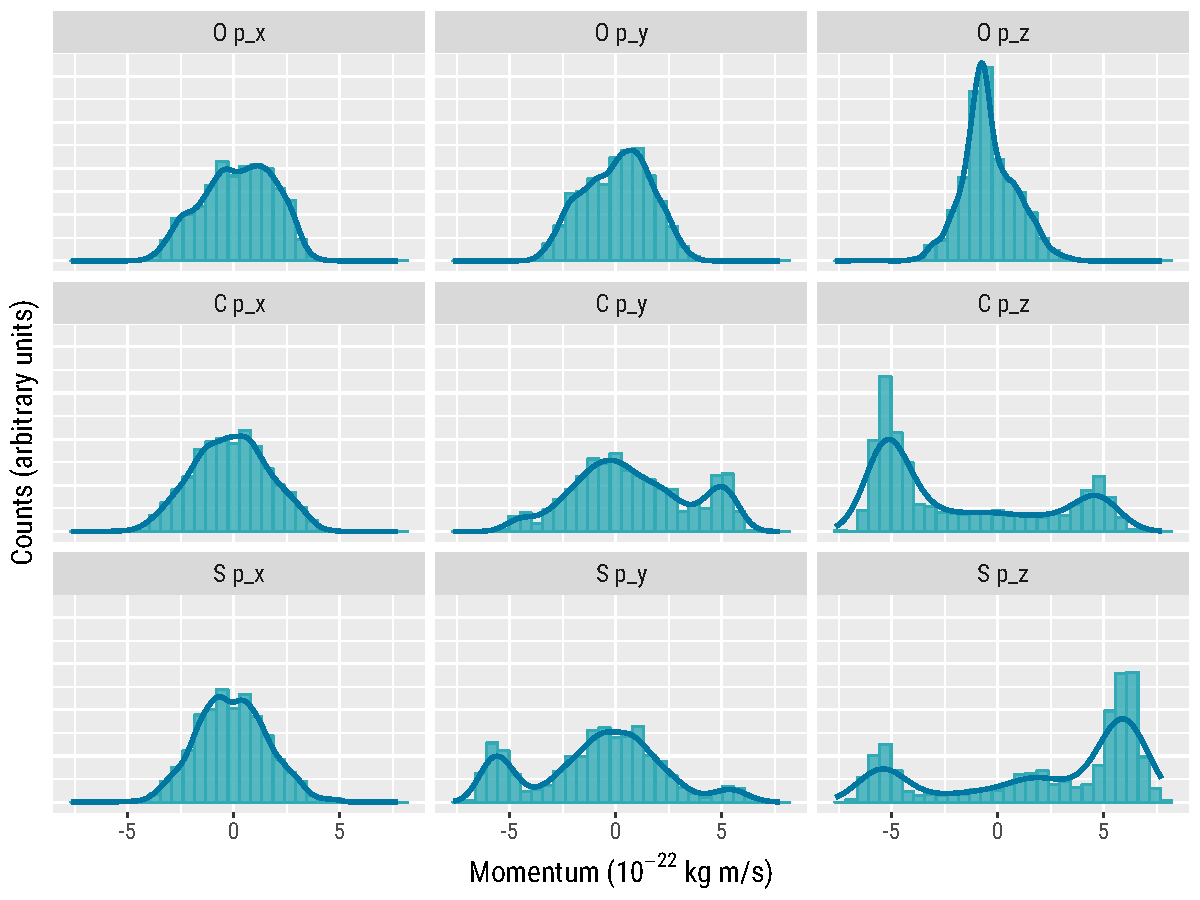
\includegraphics[width=\textwidth]{Plots/OCS22230fsMomentum}
  \caption[OCS (2,2,2) \SI{30}{\fs} momentum.]
  {OCS (2,2,2) \SI{30}{\fs} momentum.}
  \label{fig:OCS22230fsMomentum}
\end{figure}

\begin{figure}
  \centering
  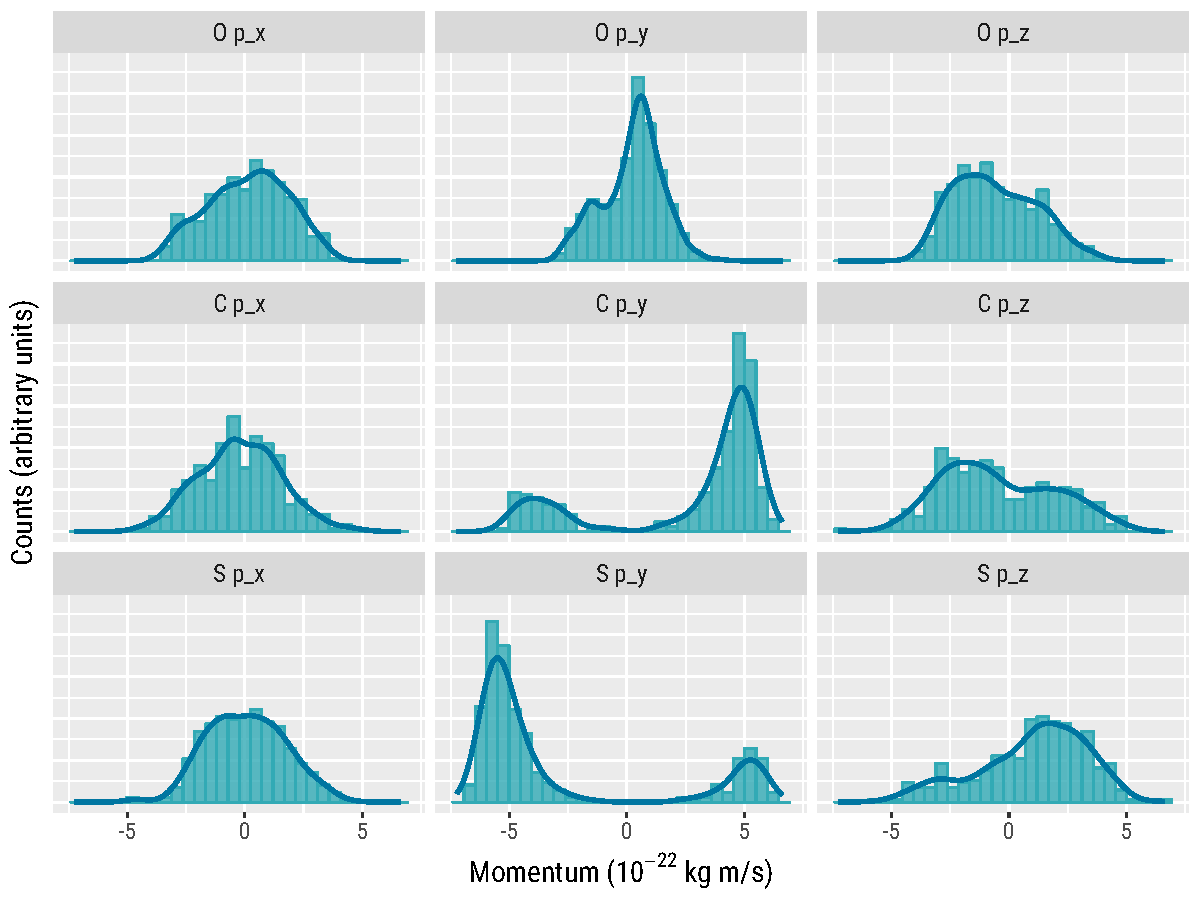
\includegraphics[width=\textwidth]{Plots/OCS22260fsMomentum}
  \caption[OCS (2,2,2) \SI{60}{\fs} momentum.]
  {OCS (2,2,2) \SI{60}{\fs} momentum.}
  \label{fig:OCS22260fsMomentum}
\end{figure}

\begin{figure}
  \centering
  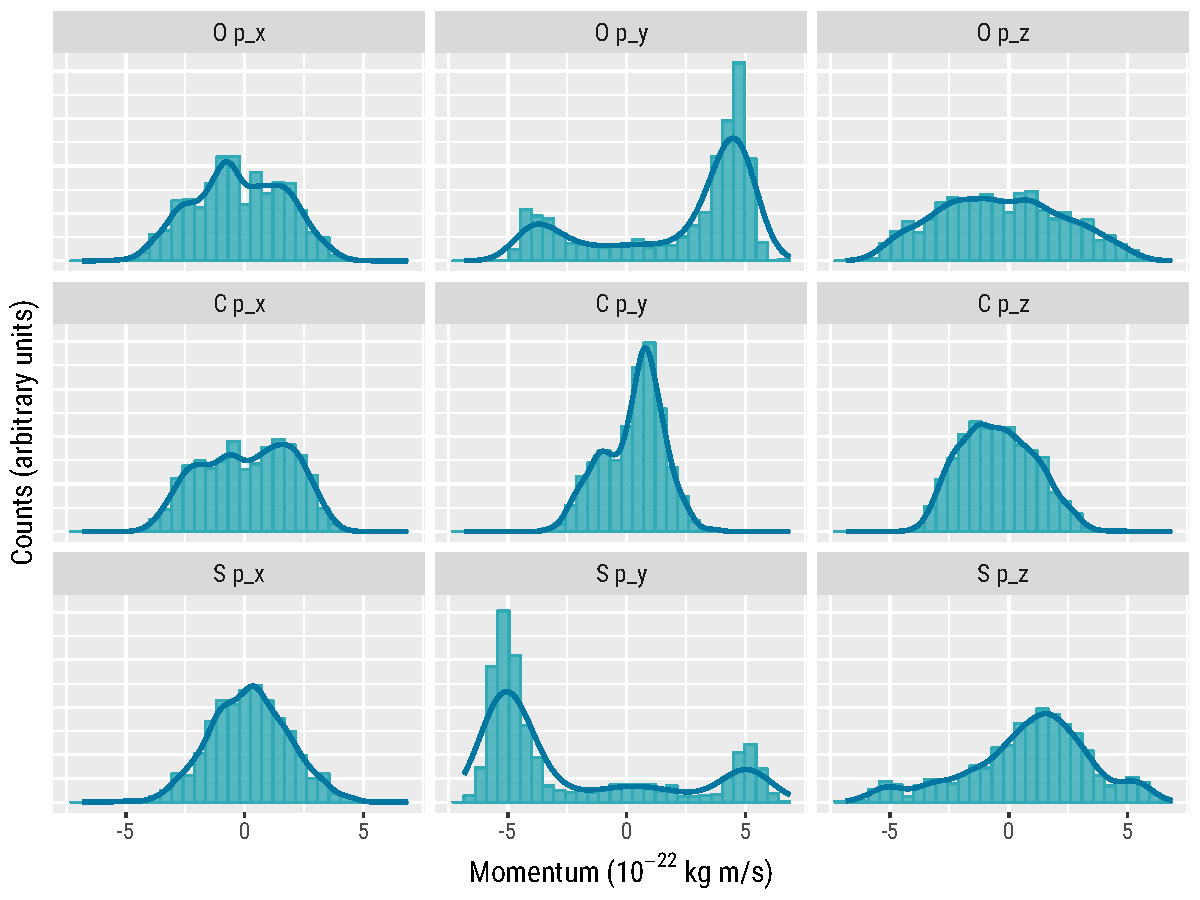
\includegraphics[width=\textwidth]{Plots/OCS222100fsMomentum}
  \caption[OCS (2,2,2) \SI{100}{\fs} momentum.]
  {OCS (2,2,2) \SI{100}{\fs} momentum.}
  \label{fig:OCS222100fsMomentum}
\end{figure}

\begin{figure}
  \centering
  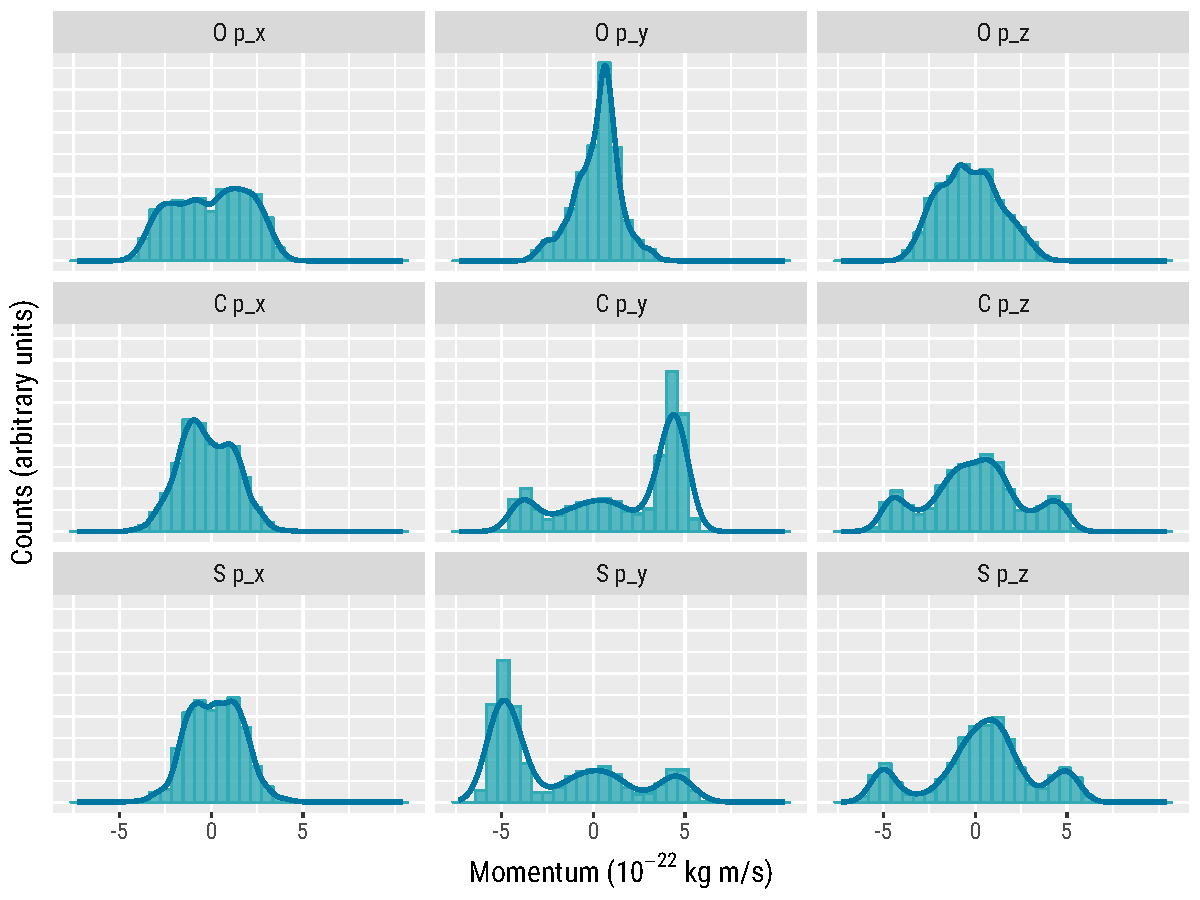
\includegraphics[width=\textwidth]{Plots/OCS222200fsMomentum}
  \caption[OCS (2,2,2) \SI{200}{\fs} momentum.]
  {OCS (2,2,2) \SI{200}{\fs} momentum.}
  \label{fig:OCS222200fsMomentum}
\end{figure}

\subsection{Momentum measurement scatter plot matrices (\SIrange{30}{200}{\femto\s})}

\begin{figure}[H]
  \centering
  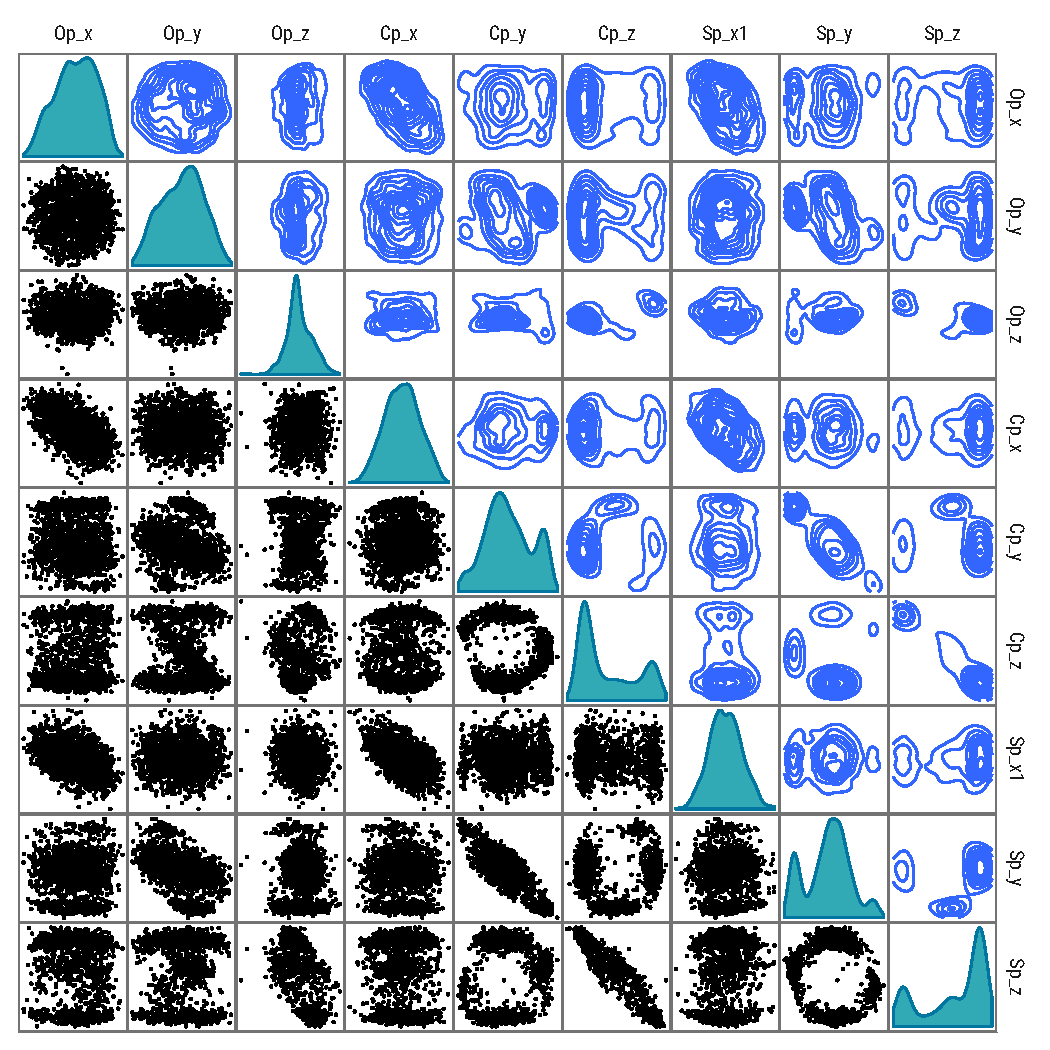
\includegraphics[width=\textwidth]{Plots/OCS22230fsMomentumPairPlots}
  \caption[OCS (2,2,2) \SI{30}{\fs} momentum pair plots.]
  {OCS (2,2,2) \SI{30}{\fs} momentum pair plots.}
  \label{fig:OCS22230fsMomentumPairPlots}
\end{figure}

\begin{figure}
  \centering
  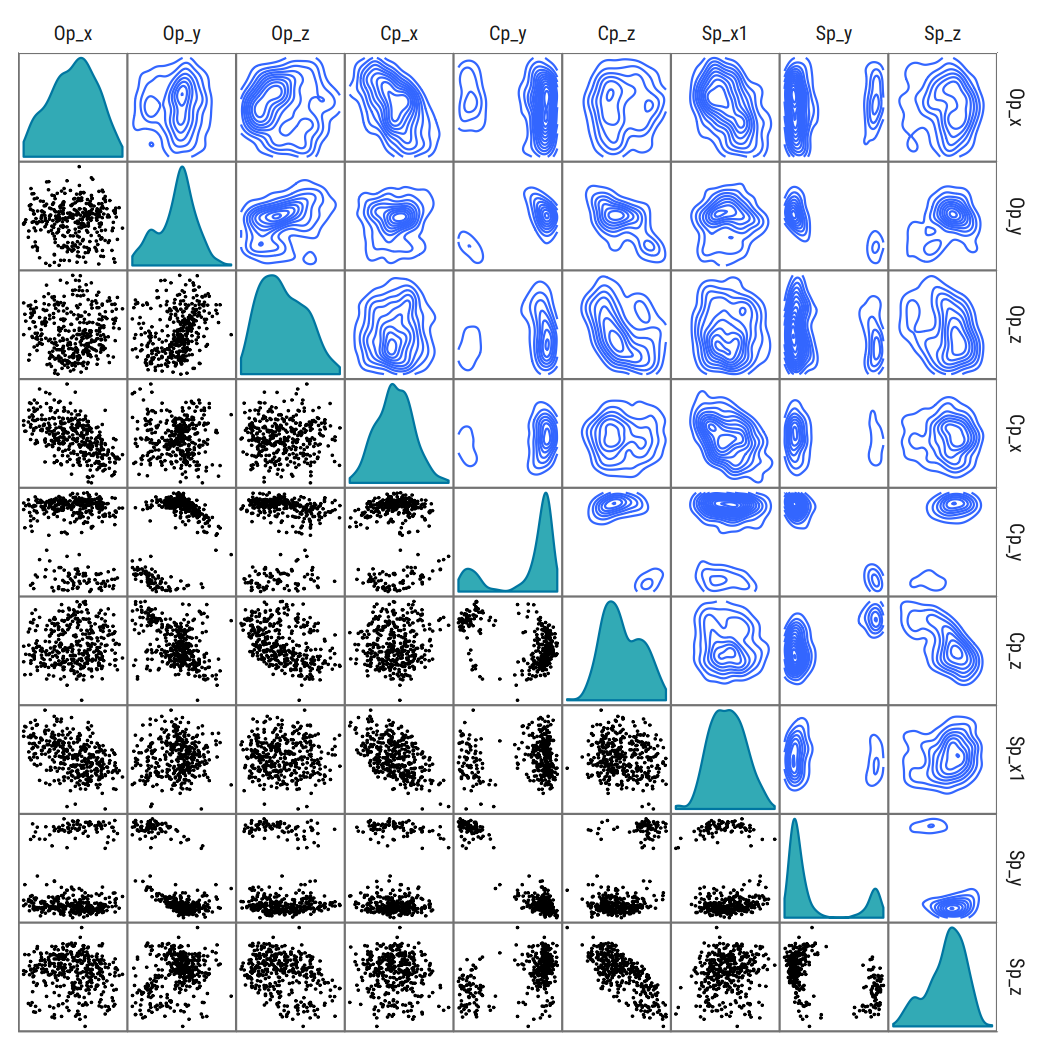
\includegraphics[width=\textwidth]{Plots/OCS22260fsMomentumPairPlots}
  \caption[OCS (2,2,2) \SI{60}{\fs} momentum pair plots.]
  {OCS (2,2,2) \SI{60}{\fs} momentum pair plots.}
  \label{fig:OCS22260fsMomentumPairPlots}
\end{figure}

\begin{figure}
  \centering
  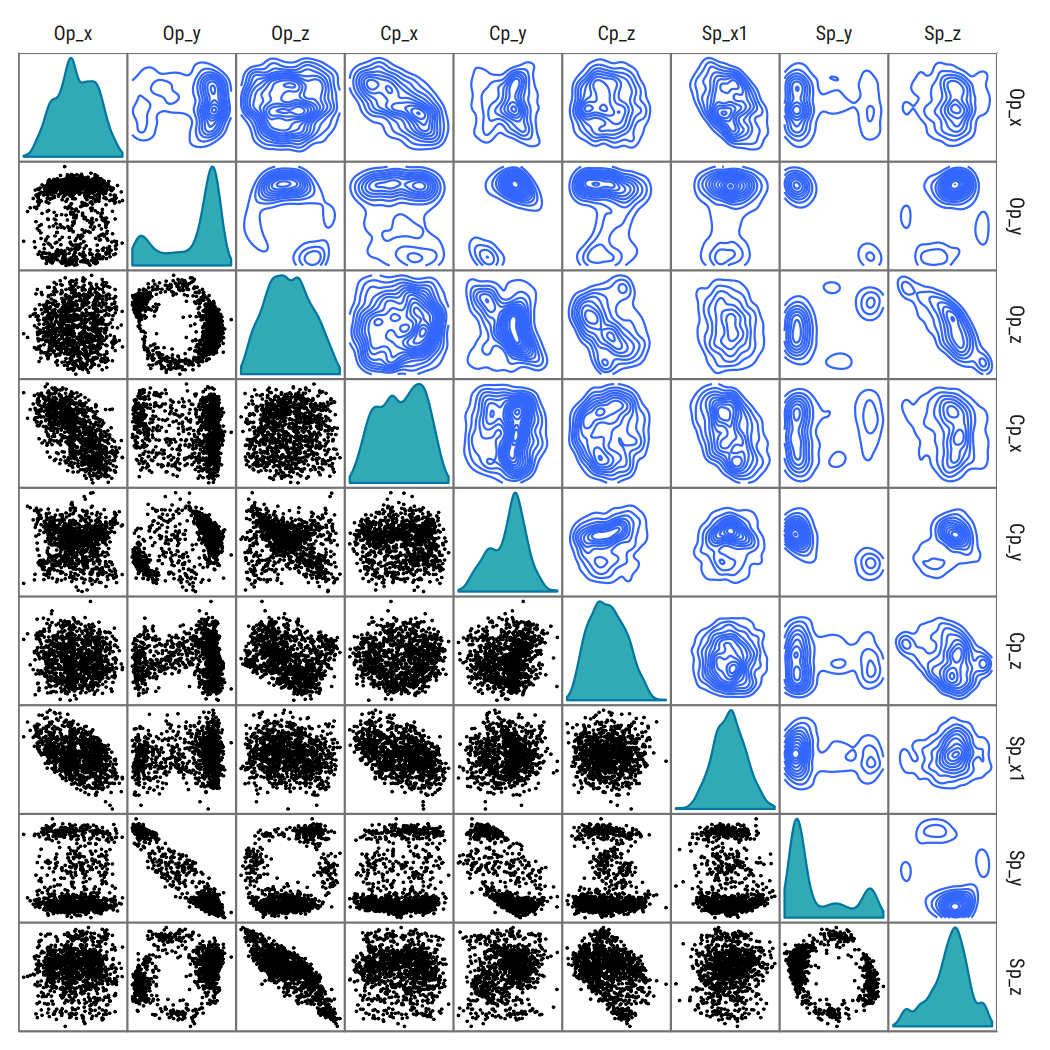
\includegraphics[width=\textwidth]{Plots/OCS222100fsMomentumPairPlots}
  \caption[OCS (2,2,2) \SI{100}{\fs} momentum pair plots.]
  {OCS (2,2,2) \SI{100}{\fs} momentum pair plots.}
  \label{fig:OCS222100fsMomentumPairPlots}
\end{figure}

\begin{figure}
  \centering
  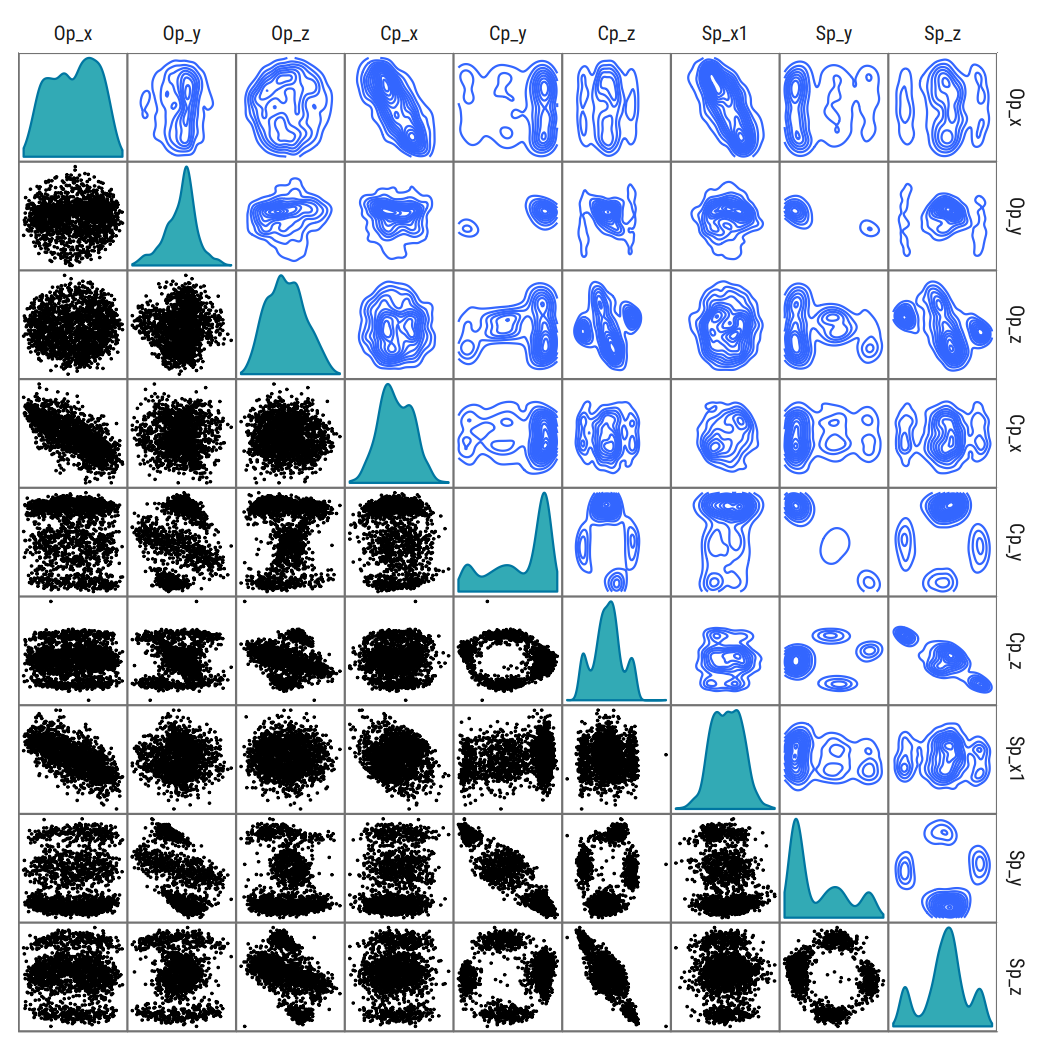
\includegraphics[width=\textwidth]{Plots/OCS222200fsMomentumPairPlots}
  \caption[OCS (2,2,2) \SI{200}{\fs} momentum pair plots.]
  {OCS (2,2,2) \SI{200}{\fs} momentum pair plots.}
  \label{fig:OCS222200fsMomentumPairPlots}
\end{figure}

\section{Lookup table geometry reconstructions}

\begin{figure}[H]
  \centering
  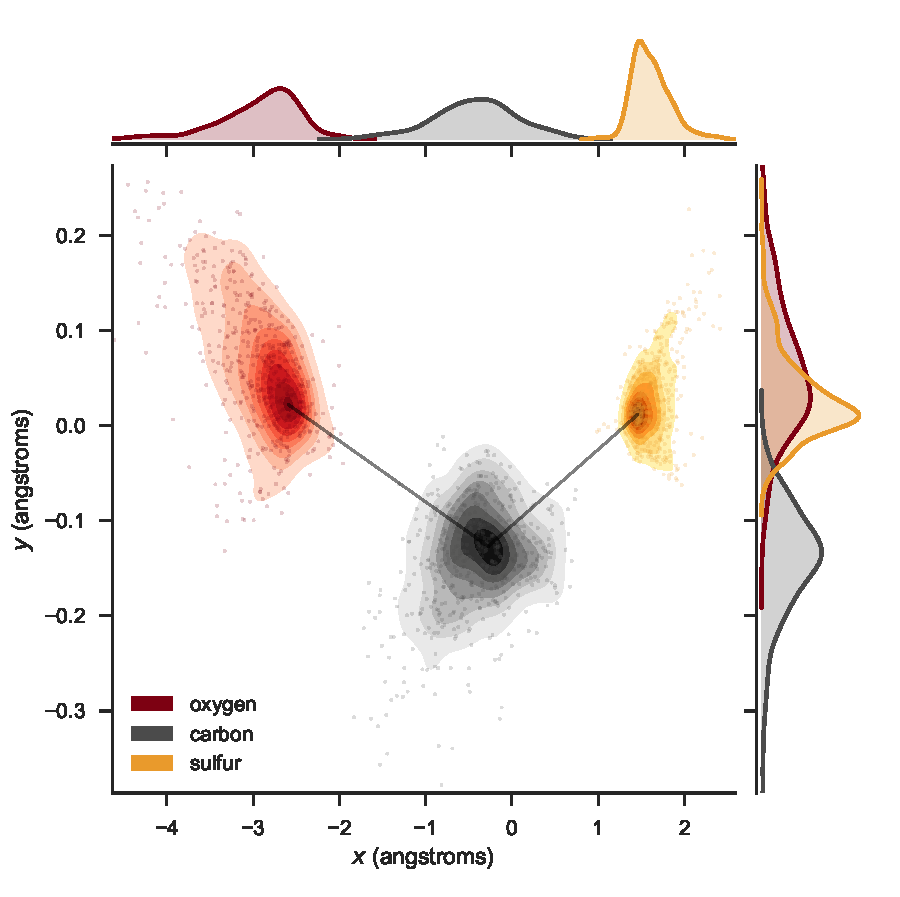
\includegraphics[width=\textwidth]{Plots/OCS22230fsLTGeometry}
  \caption[OCS (2,2,2) \SI{30}{\fs} lookup table geometry reconstruction.]
  {OCS (2,2,2) \SI{30}{\fs} lookup table geometry reconstruction.}
  \label{fig:OCS22230fsLTGeometry}
\end{figure}

\begin{figure}
  \centering
  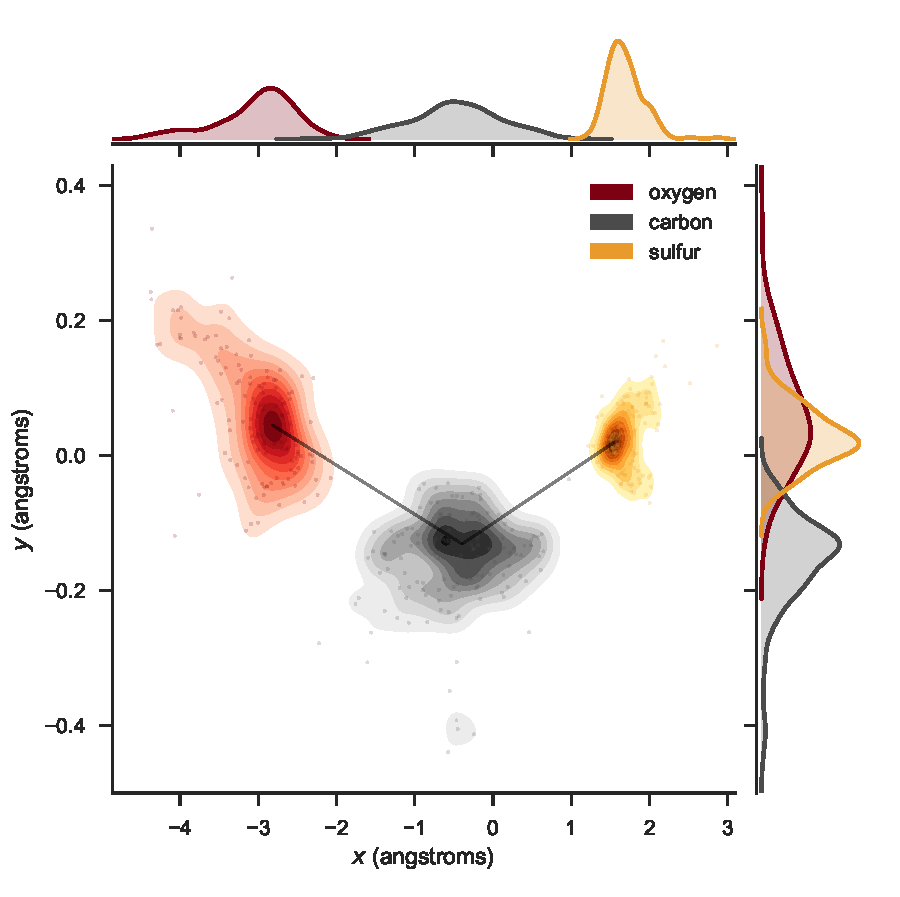
\includegraphics[width=\textwidth]{Plots/OCS22260fsLTGeometry}
  \caption[OCS (2,2,2) \SI{60}{\fs} lookup table geometry reconstruction.]
  {OCS (2,2,2) \SI{60}{\fs} lookup table geometry reconstruction.}
  \label{fig:OCS22260fsLTGeometry}
\end{figure}

\begin{figure}
  \centering
  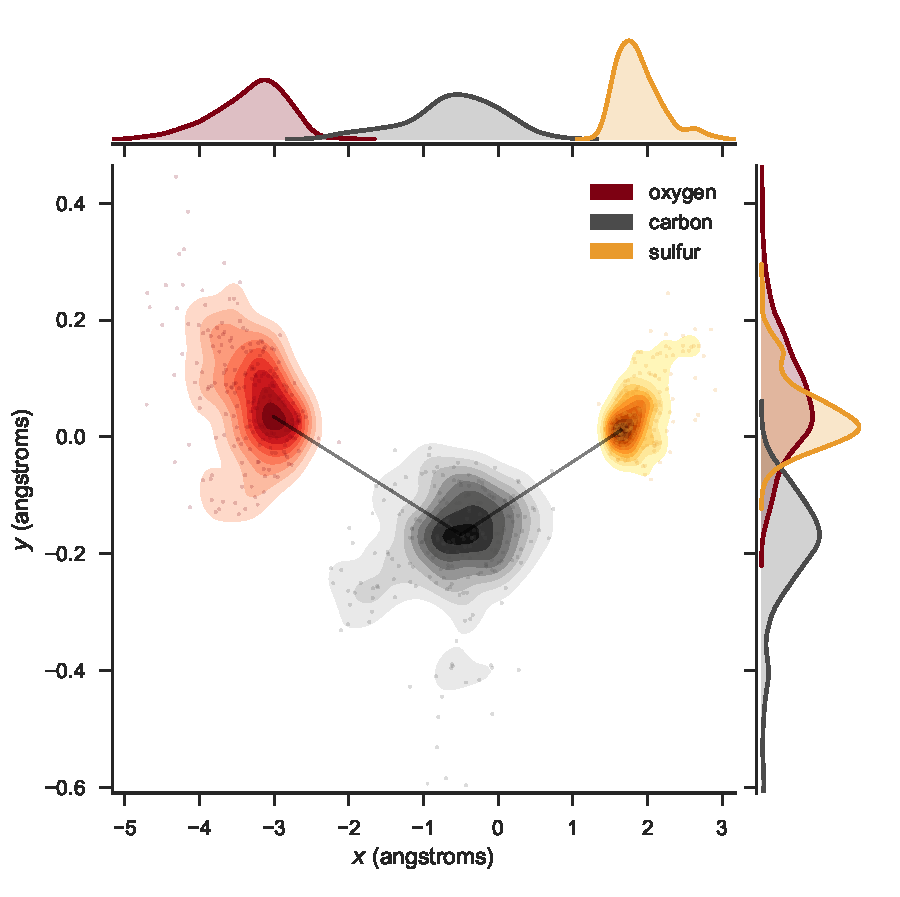
\includegraphics[width=\textwidth]{Plots/OCS222100fsLTGeometry}
  \caption[OCS (2,2,2) \SI{100}{\fs} lookup table geometry reconstruction.]
  {OCS (2,2,2) \SI{100}{\fs} lookup table geometry reconstruction.}
  \label{fig:OCS222100fsLTGeometry}
\end{figure}

\begin{figure}
  \centering
  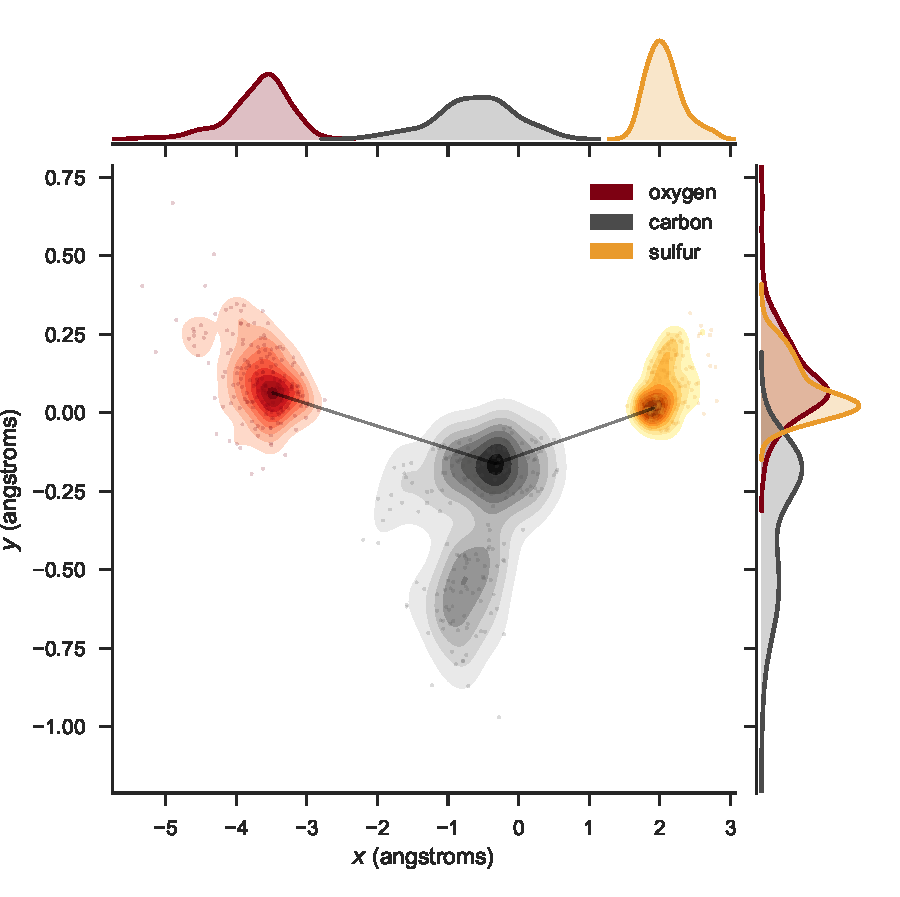
\includegraphics[width=\textwidth]{Plots/OCS222200fsLTGeometry}
  \caption[OCS (2,2,2) \SI{200}{\fs} lookup table geometry reconstruction.]
  {OCS (2,2,2) \SI{200}{\fs} lookup table geometry reconstruction.}
  \label{fig:OCS222200fsLTGeometry}
\end{figure}

\section{Mathematical optimization geometry reconstructions}

\subsection{Geometry plots}

\begin{figure}[H]
  \centering
  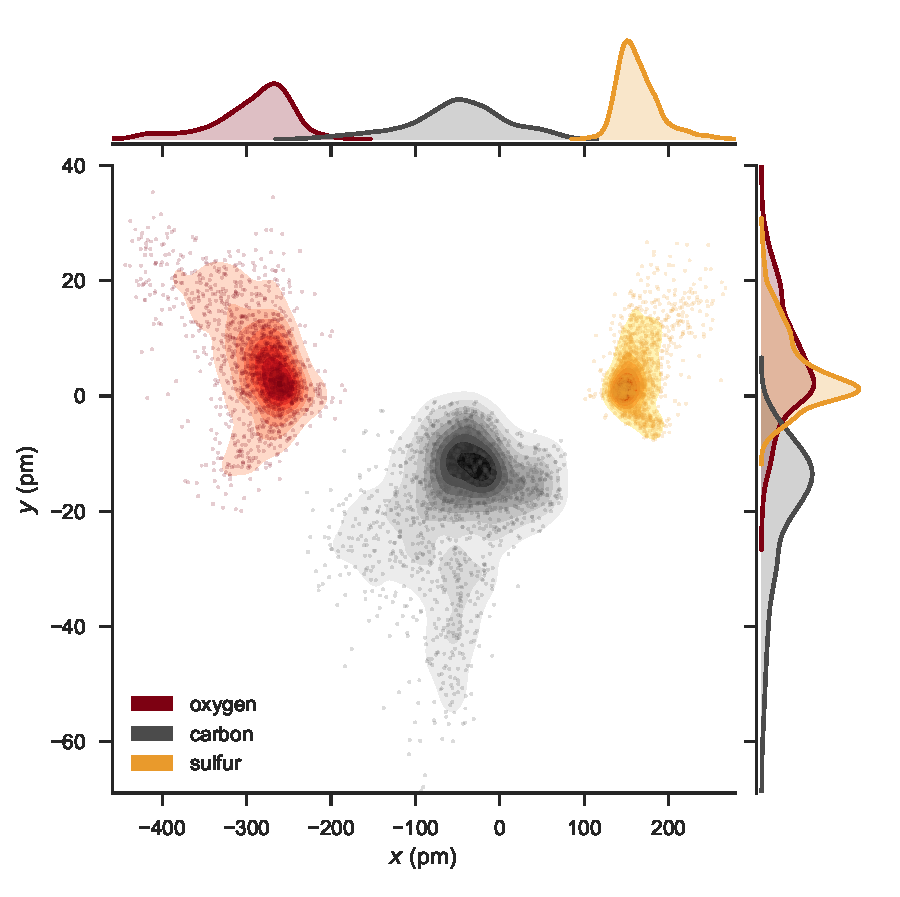
\includegraphics[width=\textwidth]{Plots/OCS22230fsMOGeometry}
  \caption[OCS (2,2,2) \SI{30}{\fs} geometry reconstructions using nonlinear constrained optimization.]
  {OCS (2,2,2) \SI{30}{\fs} geometry reconstructions using nonlinear constrained optimization.}
  \label{fig:OCS22230fsMOGeometry}
\end{figure}

\begin{figure}
  \centering
  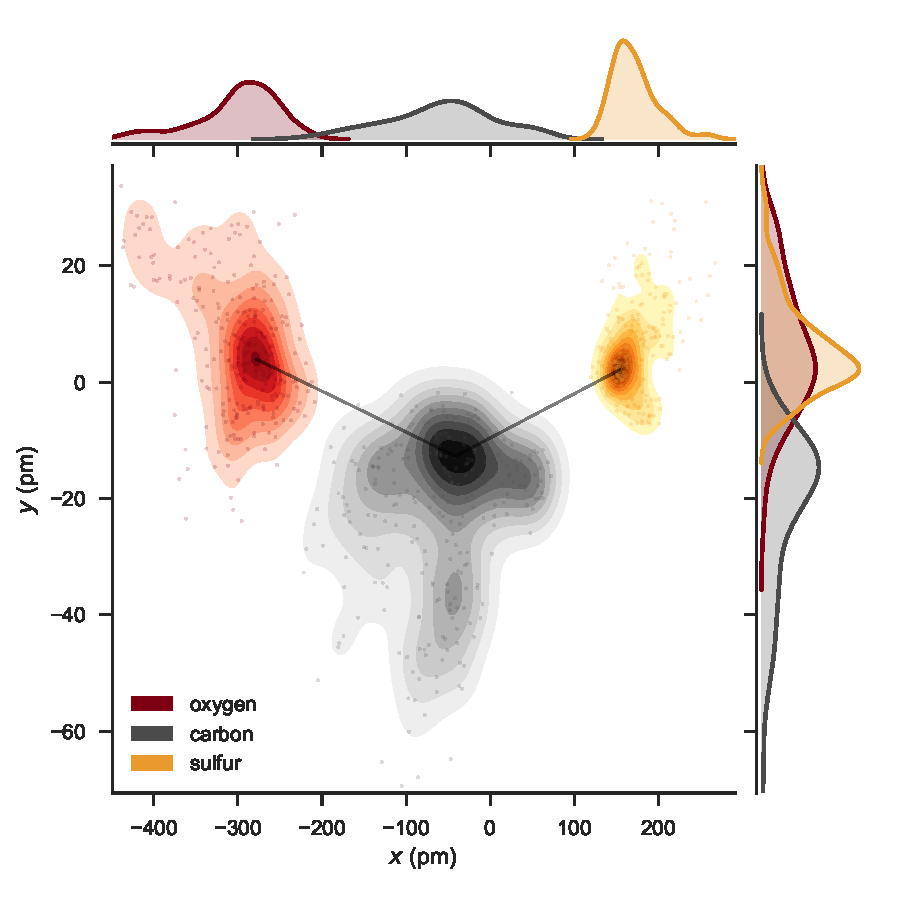
\includegraphics[width=\textwidth]{Plots/OCS22260fsMOGeometry}
  \caption[OCS (2,2,2) \SI{60}{\fs} geometry reconstructions using nonlinear constrained optimization.]
  {OCS (2,2,2) \SI{60}{\fs} geometry reconstructions using nonlinear constrained optimization.}
  \label{fig:OCS22260fsMOGeometry}
\end{figure}

\begin{figure}
  \centering
  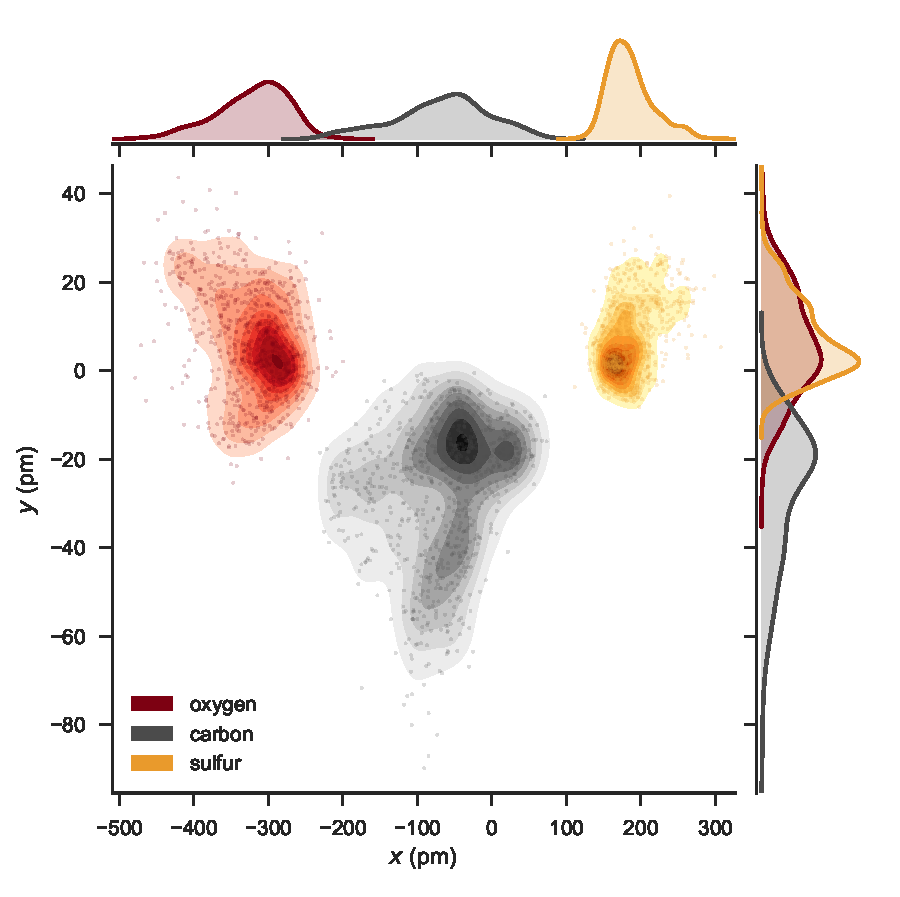
\includegraphics[width=\textwidth]{Plots/OCS222100fsMOGeometry}
  \caption[OCS (2,2,2) \SI{100}{\fs} geometry reconstructions using nonlinear constrained optimization.]
  {OCS (2,2,2) \SI{100}{\fs} geometry reconstructions using nonlinear constrained optimization.}
  \label{fig:OCS222100fsMOGeometry}
\end{figure}

\subsection{Scatter plot matrices}

\begin{figure}[H]
  \centering
  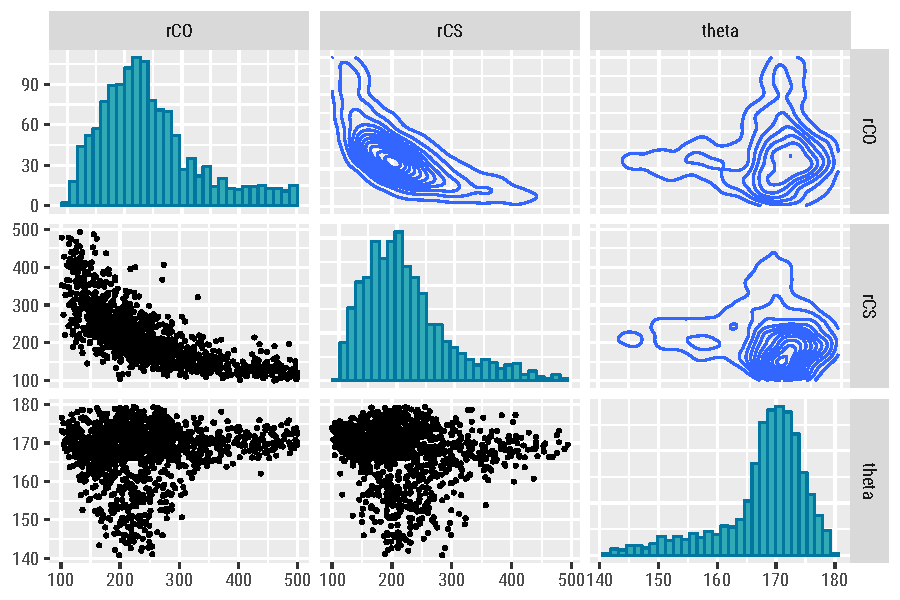
\includegraphics[width=\textwidth]{Plots/OCS22230fsMOGeometryPairs}
  \caption[Scatter plot matrices for the OCS (2,2,2) \SI{30}{\fs} geometry reconstructions using nonlinear constrained optimization.]
  {Scatter plot matrices for the OCS (2,2,2) \SI{30}{\fs} geometry reconstructions using nonlinear constrained optimization.}
  \label{fig:OCS22230fsMOGeometryPairs}
\end{figure}

\begin{figure}
  \centering
  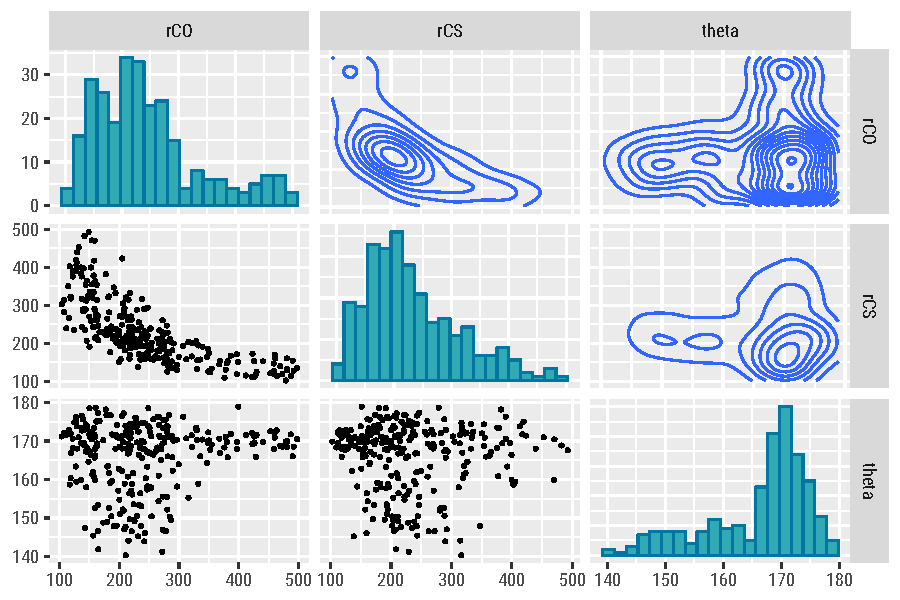
\includegraphics[width=\textwidth]{Plots/OCS22260fsMOGeometryPairs}
  \caption[Scatter plot matrices for the OCS (2,2,2) \SI{60}{\fs} geometry reconstructions using nonlinear constrained optimization.]
  {Scatter plot matrices for the OCS (2,2,2) \SI{60}{\fs} geometry reconstructions using nonlinear constrained optimization.}
  \label{fig:OCS22260fsMOGeometryPairs}
\end{figure}

\begin{figure}
  \centering
  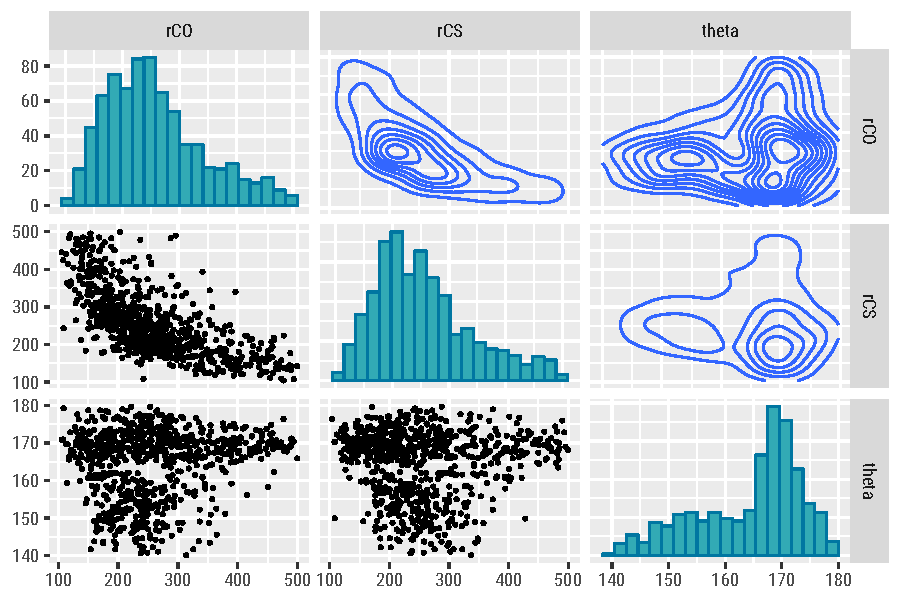
\includegraphics[width=\textwidth]{Plots/OCS222100fsMOGeometryPairs}
  \caption[Scatter plot matrices for the OCS (2,2,2) \SI{100}{\fs} geometry reconstructions using nonlinear constrained optimization.]
  {Scatter plot matrices for the OCS (2,2,2) \SI{100}{\fs} geometry reconstructions using nonlinear constrained optimization.}
  \label{fig:OCS222100fsMOGeometryPairs}
\end{figure}